\pagebreak
\subsection{Comparación PageRank vs In-Deg}

Consideremos el siguiente grafo que representa cierta web.

\begin{figure}[H]
\centering
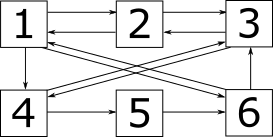
\includegraphics[scale=1]{images/grafo.png}
\caption{Caso de estudio}
\label{casoEst}
\end{figure}

Computemos el ranking de esta web utilizando PageRank ($\alpha = 0.85$) y utilizando el orden por grado de entrada.

\begin{table}[H]
\centering
\begin{tabular}{lll}
\hline
Nro. Web & PageRank & Por grado \\ \hline
1        & 0.164204 & 3         \\
2        & 0.172456 & 2         \\
3        & 0.237500 & 2         \\
4        & 0.172456 & 2         \\
5        & 0.098296 & 1         \\
6        & 0.155089 & 2         \\ \hline
\end{tabular}
\caption{PageRank vs Grado de Entrada}
\end{table}

Como podemos observar, la web con mayor ranking en PageRank es la web número 3, mientras que al utilizar el grado como medida de relevancia la web con mayor ranking es la número 1.

Intuitivamente, notemos que el algoritmo del grado ignora el hecho de que una pagina relevante que linkea a otro sitio debe contribuirle mas a su relevancia que una que otra que no es tan relevante. Este algoritmo es claramente manipulable, dado que yo puedo crear muchos sitios fácilmente que linkeen a uno que quiero favorecer en el ranking. Aquí podemos observar nuevamente una de las ventajas de PageRank, al elegir un $\alpha$ suficientemente grande, el poder de manipulación que existe es muy bajo.